
\pdfbookmark{Основное содержание работы}{content}
\section*{Основное содержание работы}

\pdfbookmark[1]{Введение}{introduction}

\highlight{Во введении} обоснована актуальность темы исследования, показана степень ее разработанности, сформулированы цель и задачи работы, приведены научная новизна, теоретическая и практическая значимость, а также положения, выносимые на защиту.

\pdfbookmark[1]{Глава 1. Проблемы создания расчетных динамических моделей конструкций по результатам модальных испытаний}{partReview}

\highlight{В первой главе} выполнен обзор методов коррекции и ассемблирования расчетных моделей. Приведены основные теоретические сведения о методах классического и операционного модального анализа. Показано, что известные методы коррекции не всегда могут быть использованы для коррекции расчетных моделей летательных аппаратов, а во многих случаях не позволяют получить достоверные результаты.

\pdfbookmark[1]{Глава 2. Коррекция и синтез расчетных динамических моделей конструкций}{partModelUpdating}

\highlight{Вторая глава} посвящена разработке и развитию методик коррекции, освобождения и синтеза расчетных динамических моделей по результатам модальных испытаний. Математическая постановка задачи коррекции допускает изменение как упругих, так и диссипативных характеристик расчетной модели. Методика коррекции основывается на дополнении исходной конечно-элементной модели внутренними и внешними корректирующими элементами. Первые определяют изменение характеристик самой модели, а вторые ответственны за коррекцию параметров внешних связей, накладываемых на модель. Корректирующие элементы строятся на узлах исходной модели. 

Рассматривается конечно-элементная модель исследуемого объекта в виде матриц жесткости $ \mat{K} $ и масс $ \mat{M} $. Собственные числа $ \lambda $ и формы колебаний $ \mat{Y} $ определяются из решения обобщённой проблемы собственных значений.

Обладая конструкторской документацией и результатами взвешивания конструкции, инерционные характеристики модели могут быть определены достаточно точно. Однако уточнение упругих характеристик модели не столь однозначно в силу совокупного объема факторов, обуславливающих погрешности моделирования: дискретизация модели, неточность задания упругих свойств материалов и граничных условий. Поэтому изменения вносятся только в матрицу жесткости путем добавления к исходной матрице $ \mat{K} $ матрицы жесткости корректирующей КЭ-модели $ \Delta \mat{K} $. Последняя записывается в виде суперпозиции матриц жесткости внутренних $ \Delta \internal{\mat{K}} $ и внешних $ \Delta \external{\mat{K}} $ корректирующих элементов.

Матрица жесткости внутреннего корректирующего элемента в общем случае имеет вид:
\begin{equation}
	\Delta \internal{\mat{K}}_j = \sum\limits_{p\,=\,1}^{q} \internal{c}_{j+p-1} \mat{G}_j^{(p)}, \ j = 1 \hdots e, \label{eq:internalStiffMatrix}
\end{equation}
где $ \internal{c}_{j+p-1} $~---~неизвестная внутренняя корректирующая жесткость; $ q $~---~число внутренних корректирующих жесткостей, описывающих элемент; $ \mat{G}_j^{(p)} $~---~парциальная матрица жесткости внутреннего коррректирующего элемента; $ e $~---~число внутренних корректирующих элементов. 

Число корректирующих жесткостей $ q $ зависит от числа физических параметров, которыми описывается добавляемый элемент. Для коррекции модели, составленной из объемных элементов, в качестве корректирующей КЭ-модели используется ферменная конструкция ($ q = 1 $). В случае, если динамические свойства модели существенно зависят от изгибных и крутильных жесткостей её балочных или оболочечных элементов, предлагается использовать корректирующую КЭ-модель из балочных элементов ($ q = 4 $). 

В качестве внешних корректирующих элементов используются пружинные опоры, прикрепленные к неподвижному основанию. Матрица $ \Delta \external{\mat{K}} $ имеет следующий вид:
\begin{equation}
	\Delta \external{\mat{K}} = \operatorname{diag} \cbrackets{\external{c}_1, \external{c}_2, \hdots, \external{c}_N}, \label{eq:externalStiffMatrix}
\end{equation}
где $ N $~---~размерность КЭ-модели, $ \external{\mat{c}} $~---~неизвестные внешние корректирующие жесткости. 

Рассматривается итерационный алгоритм коррекции, позволяющий избежать многократного решения обобщенной проблемы собственных значений. На каждом шаге коррекции жесткости корректирующих элементов являются неизвестными параметрами $ \mat{c} = \rbrackets{\internal{\mat{c}}, \external{\mat{c}}} $, которые определяются из решения задачи безусловной минимизации целевой функции:
\begin{gather}
	\sum\limits_{i = 1} ^ s w_i \sbrackets{\trans{\rbrackets{\mat{Y}_i ^ {(j)}}} \Delta \mat{K} ^ {(j + 1)} \mat{Y}_i ^ {(j)} - \Delta \lambda_i ^ {(j + 1) \ast} \trans{\rbrackets{\mat{Y}_i ^ {(j)}}} \mat{M} \mat{Y}_i ^ {(j)}} ^ 2 \rightarrow \min_{\mat{c}},
\end{gather}
где $ s $~---~целевое число корректируемых тонов, $ j $~---~номер итерации, $ \Delta \lambda_i ^ {\ast}$~---~разница между текущими и целевыми собственными значениями $ i $-го тона, $ w_i $~---~весовой коэффициент $ i $-го тона.

Для решения задачи минимизации целевой функции применяется метод сопряженных градиентов. Используются аналитические выражения для компонент вектора-градиента целевой функции, что позволяет кратно сократить время, потребное для осуществления коррекции. Кроме того, исключается необходимость определения оптимального шага численного дифференцирования.

На рисунке~\ref{fig:principalSchemeUpdating} приведена принципиальная схема, иллюстрирующая физическую сторону предлагаемой методики на примере простой модели летательного аппарата. В данном случае модель составлена из объемных и оболочечных элементов, поэтому для изменения её динамических свойств вводятся как балочные, так и ферменные корректирующие элементы. Кроме того, для описания модели упругого основания, вводятся пружинные элементы. Таким образом, корректирующая модель образует <<каркасную>> структуру над исходной моделью.

\begin{figure}[H]
	\centerfloat
	\begin{tikzpicture}[scale = 0.7]
		\pgfmathsetmacro{\nodeDist}{0.1}
		\pgfmathsetmacro{\shiftText}{0.0}
		% Исходная модель
		\node[inner sep = 0pt] (initial) at (0, 0) {\includegraphics[width = 0.3\textwidth]{simple-model-initial}};
		\node[inner sep = 0pt, below = \shiftText of initial.south] (textInitial) {Исходная модель};
		% Знак
		\node [below = \nodeDist of textInitial.south, color = blue] (sumSign) {\Huge \bfseries +};
		% Коррректирующие элементы
		\node[inner sep = 0pt, below = -\nodeDist of sumSign.south] (elements) {\includegraphics[width = 0.3\textwidth]{simple-model-elements}};
		\node[inner sep = 0pt, below = \shiftText of elements.south] (textElements) {Корректирующие элементы};
		% Скорректированная модель
		\draw [-{Latex[length = 4mm]}, color = red, ultra thick](sumSign.east) ++ (3, 0) --++ (1.25, 0) node [right] (updated) {\includegraphics[width = 0.4\textwidth]{simple-model-updated}};
		\node[inner sep = 0pt, below = \shiftText of updated.south] (textUpdated) {Скорректированная модель};
	\end{tikzpicture}
	\caption{Принципиальная схема коррекции} \label{fig:principalSchemeUpdating}
\end{figure}

Набор корректирующих элементов формируется автоматически на основе портрет матрицы жесткости корректируемой конструкции. В общем случае число таких корректирующих элементов определяется количеством связей между узлами в матрице, но оно может быть уменьшено посредством выбора областей коррекции, например, элементов конструкции с наибольшей неопределенностью физических и геометрических характеристик. 

Полагаем, что по экспериментальным соотношениям между монофазными и собственными колебаниями подтверждено, что матрица демпфирования в главных координатах имеет диагональный вид. Тогда известны $ s $ обобщенных коэффициентов демпфирования $ \mat{h} ^ \ast $, которые определены по результатам экспериментального модального анализа. Матрица демпфирования в физической системе координат строится в два этапа: в качестве нулевого приближения используется гипотеза Е.\,С.~Сорокина, а затем, для достижения целевых обобщенных коэффициентов демпфирования вводятся корректирующие элементы.

Нулевое приближение матрицы демпфирования имеет вид:
\begin{equation}
	\mat{H} = \alpha \mat{K} ^ \ast + \beta \mat{M},
\end{equation}
где $ \mat{K} ^ \ast $~---~скорректированная матрица жесткости, $ \alpha $~---~коэффициент конструкционного демпфирования, $ \beta $~---~коэффициент инерционного демпфирования.

Собственные частоты и формы колебаний, вычисленные в результате решения обобщенной проблемы, остаются неизменными в процессе восстановления матрицы демпфирования. Обобщенные жесткости $ \kappa_i $ и массы $ \mu_i $ целевых тонов колебаний используются для определения коэффициентов $ \alpha $ и $ \beta $ в результате решения задачи минимизации целевой функции:
\begin{equation}
	\sum \limits_{i\,=\,1} ^ s w_i \left( 1 - \frac{\alpha \kappa_i + \beta \mu_i}{h_i ^ \ast} \right)^2 \rightarrow \min_{\alpha, \beta}.
\end{equation}

По аналогии с~\eqref{eq:internalStiffMatrix} и \eqref{eq:externalStiffMatrix} нулевое приближение матрицы демпфирования уточняется введением корректирующих элементов:
\begin{equation}
	\tilde{\mat{H}} = \mat{H} + \Delta \internal{\mat{H}} + \Delta \external{\mat{H}},
\end{equation}
где $ \Delta \internal{\mat{H}} $ и $ \Delta \external{\mat{H}} $~---~матрицы демпфирования внутренних и внешних корректирующих элементов. Под внутренним демпфированием понимаются потери энергии за счет трения в материалах модели, а под внешним~---~рассеяние энергии при взаимодействии модели с окружающей средой, например, воздухом. Последнее особенно актуально для крупногабаритных конструкций.

Алгоритм восстановления матрицы демпфирования заключается в том, чтобы найти такие параметры $ \eta_1, \eta_2, \hdots, \eta_m $, которые будут решением следующей недоопределенной системы нелинейных уравнений:
\begin{equation}
	f_i = \trans{\rbrackets{\mat{Y}_i ^ \ast}} \tilde{\mat{H}} \mat{Y}_i ^ \ast - h_i ^ \ast, \ i = 1 \hdots s. \label{eq:systemDampUpdating}
\end{equation}

Решением системы~\eqref{eq:systemDampUpdating} считается решение задачи безусловной минимизации целевой функции, равной сумме квадратов каждого из уравнений с взвешенной суммой квадратов коэффициентов демпфирования:
\begin{equation}
	\sum \limits_{i\,=\,1} ^ s w_i f_i ^ 2 + w_c \sum \limits_{i\,=\,1}^s \eta_i ^ 2 \rightarrow \min_\mat{\eta},
	\label{eq:objFinalDampFunUpdating}
\end{equation}
где $ w_i $~---~весовые коэффициенты корректируемых тонов, $ w_c $~---~параметр регуляризации.

Важно отметить, что расчетной моделью летательного аппарата является модель свободной динамической системы. В то же время для модальных испытаний авиационная техника либо устанавливается на шасси, либо помещается на специальную систему упругого вывешивания, а космические конструкции~---~на систему обезвешивания. Системы упругого вывешивания и обезвешивания, влияние которых на свободную конструкцию строго регламентировано, являются сложными и дорогостоящими техническими сооружениями. Поэтому разработана методика освобождения скорректированной КЭ-модели от закреплений, наложенных для проведения экспериментов. Предположено, что информации об убранных при начальном закреплении модели степенях свободы либо нет, либо она неактуальна, то есть она не позволяет сделать модель свободной.

Суть методики освобождения заключается в том, что матрицы жесткости и масс расширяются шестью степенями свободы $ \mat{\xi} $, которые отвечают за перемещения и повороты модели как жесткого целого. Дополнительные элементы матриц рассчитываются следующим образом:
\begin{equation}
	\begin{pmatrix}
		\mat{K} & -\trans{\rbrackets{\sum \mat{k}}} \\
		 -\sum \mat{k} & \kappa + \sum \sum \mat{k}
	\end{pmatrix}
	\begin{Bmatrix}
		\tilde{\mat{Y}} \\
		\xi
	\end{Bmatrix}
	+
	\begin{pmatrix}
		\mat{M} & \mat{0} \\
		\mat{0} & \mu - \sum \sum \mat{m}
	\end{pmatrix}
		\begin{Bmatrix}
		\ddot{\tilde{\mat{Y}}} \\
		\ddot{\xi}
	\end{Bmatrix}
	= 0,
\end{equation}
где $ \sum \mat{k} \in \set{R}^{6 \times n}$, $ \sum \mat{m} \in \set{R}^{6 \times n}$, $ \sum \sum \mat{m} \in \set{R}^{6 \times 6} $~---~дополнительные матричные элементы; $ \tilde{\mat{Y}} $~---~вектор узловых перемещений относительно некоторой точки, например, центра тяжести.

Описано использование метода статистического моделирования для оценки устойчивости результата коррекции к погрешностям в значениях частот, определенных экспериментально. Суть метода состоит во внесении случайных отклонений в исходные значения частот собственных колебаний с последующей оценкой искажений форм колебаний по критерию модального соответствия $ \varepsilon_{\mathrm{MAC}} $. Для моделирования ошибок $\Delta \mat{f} $ используется генератор случайных чисел, имеющих усеченное нормальное распределение. Концы этого распределения совмещены с предельным шумовым уровнем и соответствуют утроенному среднеквадратическому отклонению. 

На примере свободной прямоугольной пластины показаны зависимости искажений форм колебаний относительно ошибок в целевых частотах, полученные при разном числе корректируемых тонов собственных колебаний~\figref{fig:perturbation-plate-errors}. При этом точки, составляющие эти зависимости, определены путем многократного проведения независимых испытаний на одном уровне шума. Число этих испытаний $ N_\Sigma $, которое потребовалось для стабилизации центрального момента критерия модального соответствия, приведено на рисунке~\ref{fig:perturbation-plate-samplesize}. Видно, что методика устойчива во всем диапазоне вносимых отклонений. Более того, при увеличении числа тонов кривые стремятся к предельной огибающей. Аналогичный результат получен для более сложной конструкции~---~тестовой модели космического аппарата.

\begin{figure}[!htb]
\centering
\vspace{-1em}
\begin{minipage}[b]{0.49\textwidth}
	\centering
	\begin{tikzpicture}[scale = 1]
		\begin{semilogyaxis}[
			xlabel           = {$\Delta \mat{f} $, \% },
			ylabel           = {$ \varepsilon_{\mathrm{MAC}} $, \%},
			ylabel shift     = -2 pt,
			grid             = major,
			legend columns   = 2,
			legend style     = {
				at           = {(0.76, 0.03)},
				anchor       = south,
				fill         = white,
				fill opacity = 0.6,
				draw opacity = 1,
				text opacity = 1,
			},
			ylabel near ticks,  
			xtick            = {0, 1, 2, 3, 4, 5},
			ytick            = {1e-6, 1e-4, 1e-2, 1e0},
			mark size        = 1pt,
			width            = 6.4cm
		]
			\pgfplotstableread{images/partModelUpdating/perturbation-plate-errors.txt}\contentFile
			\addplot[color = blue, mark = *] table [x index = 0, y index = 1] {\contentFile};
			\addplot[color = red, mark = triangle*] table [x index = 0, y index = 2] {\contentFile};
			\addplot[color = olive, mark = diamond*] table [x index = 0, y index = 3] {\contentFile};
			\addplot[color = purple, mark = halfcircle*] table [x index = 0, y index = 4] {\contentFile};
			\addplot[color = teal, mark = x] table [x index = 0, y index = 5] {\contentFile};
			\legend{$ 1 $, $ 3 $, $ 5 $, $ 7 $, $ 9 $}
		\end{semilogyaxis}
	\end{tikzpicture}
	\caption{Погрешность определения форм колебаний пластины} \label{fig:perturbation-plate-errors}
\end{minipage}
\hfill
\begin{minipage}[b]{0.49\textwidth}
	\centering
	\begin{tikzpicture}[scale = 1]
		\begin{axis}[
			xlabel           = {$\Delta \mat{f} $, \% },
			ylabel           = {$ N_\Sigma $},
			ylabel shift     = -5 pt,
			legend columns   = 1,
			legend style     = {
				at           = {(0.05, 0.68)},
				anchor       = west,
				fill         = white,
				fill opacity = 0.6,
				draw opacity = 1,
				text opacity = 1,
			},
			ylabel near ticks,
			try min ticks = 6,
			bar width  = 2pt,
			width      = 6.4cm,
			ybar stacked,
			scaled y ticks = base 10:-3,
          	xmin = 0.15, xmax = 5.05, ymin = 0
		]
			\pgfplotstableread{images/partModelUpdating/perturbation-plate-samplesize.txt}\contentFile
			\addplot table [x index = 0, y index = 1] {\contentFile};
			\addplot table [x index = 0, y index = 2] {\contentFile};
			\addplot table [x index = 0, y index = 3] {\contentFile};
			\addplot table [x index = 0, y index = 4] {\contentFile};
			\addplot table [x index = 0, y index = 5] {\contentFile};
			\legend{$ 1 $, $ 3 $, $ 5 $, $ 7 $, $ 9 $}
		\end{axis}
	\end{tikzpicture}
	\caption{Число независимых испытаний пластины} \label{fig:perturbation-plate-samplesize}
\end{minipage}
\end{figure}

Развита методика, состоящая в декомпозиции крупногабаритных трансформируемых конструкций на составные части, которые подвергаются модальным испытаниям независимо друг от друга. Результаты испытаний используются для коррекции, освобождения и синтеза расчетных моделей составных частей~\figref{fig:schemeDecomposition}. Обоснован выбор граничных условий в испытаниях составных частей. Кроме того, имея в виду достижение физической согласованности скорректированных моделей, предложено использовать результаты нескольких экспериментов при различных условиях закрепления одной составной части.

\begin{figure}[!htb]
	\centering
	\begin{subfigure}[b]{0.45\textwidth}
		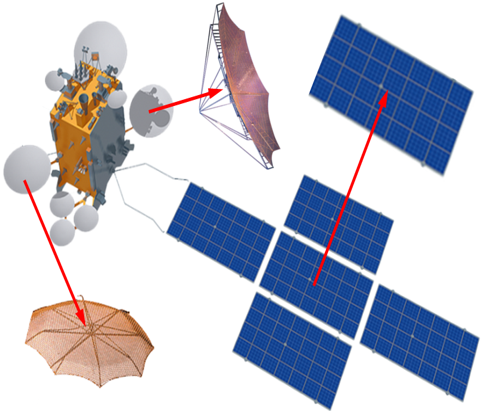
\includegraphics[width = \textwidth]{decomposition}
	\end{subfigure}
	\hfill
	\begin{subfigure}[b]{0.45\textwidth}
	     % Определение стиля
        \tikzstyle{blockWide} = [rectangle, draw = black, fill = blue!15, rounded corners, text width = 20em, text centered, minimum height = 1.5em, drop shadow] 
        \tikzstyle{blockWideC} = [blockWide, fill = red!20]
        \tikzstyle{arrow} = [draw, thick, color = black!90, -latex'] 
        \scriptsize 
        % Задание перменных
        \def\nodeDist{0.3cm}
        % Отрисовка блок-схемы
        \begin{tikzpicture}[scale = 1, transform shape]
            % Задание узлов		
            \node (modalTests) [blockWide] {Модальные испытания \\ составных частей конструкции};
            \node (modelUpdating) [blockWide, below = \nodeDist of modalTests] {Коррекция расчетных моделей \\ составных частей  конструкции \\ по результатам испытаний};
            \node (checkInfluence) [blockWide, below = \nodeDist of modelUpdating] {Освобождение расчетных моделей \\ составных частей конструкции};
            \node (buildRealModel) [blockWide, below = \nodeDist of checkInfluence] {Синтез расчетной модели полной \\ конструкции из её составных частей};
            \node (buildMathModel) [blockWide, below = \nodeDist of buildRealModel] {Определение динамических \\ характеристик полной расчетной модели};
            % Соединение узлов
            \draw [arrow] (modalTests.south) -- (modelUpdating.north);
            \draw [arrow] (modelUpdating.south) -- (checkInfluence.north);
            \draw [arrow] (checkInfluence.south) -- (buildRealModel.north);
            \draw [arrow] (buildRealModel.south) -- (buildMathModel.north);
        \end{tikzpicture}
	\end{subfigure}
    \caption{Схема методики синтеза расчетных моделей крупногабаритных трансформируемых конструкций} \label{fig:schemeDecomposition}
    \vspace{1em}
\end{figure}  

Методика синтеза протестирована на примере упрощенной модели космического аппарата, состоящего из орбитального модуля и панелей солнечных батарей. Каждая составная часть корректировалась по девяти частотам собственных колебаний, используя данных двух виртуальных экспериментов. Максимальная погрешность в определении первых шестнадцати частот синтезированной модели до коррекции равнялась $ 5.121 $ \%, а после коррекции составила $ 0.1 $ \%. Распределение изменений узловых жесткостей по всем линейным степеням свободы для моделей составных частей до и после коррекции показано на рисунке~\ref{fig:test-spacecraft-distribution}. 

\begin{figure}[H]
	\centering
	\vspace{-1.5em}
	\begin{subfigure}[t]{0.46\textwidth}
		\centering
		\includegraphics[width = \textwidth]{test-spacecraft-orbital-distribution}
		\caption{\small Орбитальный модуль} \label{subfig:test-orbital-distribution}
	\end{subfigure}
	\hfill
	\begin{subfigure}[t]{0.44\textwidth}
		\centering
		\includegraphics[height = \textwidth]{test-spacecraft-panel-distribution}
		\caption{\small Панели солнечных батарей} \label{subfig:test-panel-distribution}
	\end{subfigure}
	\vspace{1em}
	\caption{Изменения узловых жесткостей при коррекции моделей составных частей} \label{fig:test-spacecraft-distribution} 
\end{figure}

\pdfbookmark[1]{Глава 3. Результаты модальных испытаний как исходные данные для коррекции расчетных моделей конструкций}{partModalAnalysis}

\highlight{В третьей главе} развиваются методы классического и операционного модального анализа, позволяющие получать достоверные оценки динамических параметров для коррекции. С целью обеспечения возможности эффективного расчета обобщенных характеристик по результатам модальных испытаний, составлена программная реализация, позволяющая посредством графического интерфейса~\figref{subfig:gencalc-interface} гибко менять параметры расчета и исследовать зависимости получаемых характеристик несколькими способами одновременно. 

Одним из ключевых требований обеспечения непрерывности производственного процесса авиационной техники является сокращение времени между натурными испытаниями и первым вылетом изделия. Поэтому разработана программа~\figref{subfig:analyzer-interface}, использующая программный интерфейс \name{Testlab Automation} для обработки и представления результатов модального анализа непосредственно в процессе испытаний.

\begin{figure}[!htb]
	\centering
	\begin{subfigure}[t]{0.45\textwidth}
		\centering
		\includegraphics[width = \textwidth]{gencalc-interface}
		\caption{\small Определение модальных параметров} \label{subfig:gencalc-interface}
	\end{subfigure}
	\hfill
	\begin{subfigure}[t]{0.52\textwidth}
		\centering
		\includegraphics[width = \textwidth]{analyzer-interface}
		\caption{\small Экспресс-представление результатов} \label{subfig:analyzer-interface}
	\end{subfigure}
	\vspace{1em}
	\caption{Программы для обработки и представления результатов модальных испытаний} 
\end{figure}

Изложена методика контроля зазоров в технических изделиях по искажениям портретов вынужденных колебаний в процессе вибрационных испытаний. Представлен способ поэтапного выявления всех зазоров в объекте испытаний, которые приводят к искажениям портретов колебаний. В рамках описываемого подхода разработана и введена в программное обеспечение управления испытаниями подпрограмма анализа портретов колебаний. Методика обнаружения зазоров по искажениям портретов колебаний использована для диагностирования самолётов в процессе модальных испытаний~\figref{fig:distortion-wiring-backlash}, а также космических аппаратов открытого исполнения в технологических вибрационных испытаниях~\figref{fig:distortion-spacecraft}. 

\begin{figure}[!htb]
	\centering
	\begin{minipage}{0.59\textwidth}
		\centering
		\includegraphics[width = \linewidth]{distortion-wiring-backlash} 
		\captionof{figure}{Люфт в соединении ручки управления с проводкой} \label{fig:distortion-wiring-backlash}
	\end{minipage}
	\hfill
	\begin{minipage}{0.4\textwidth}
		\centering
		\includegraphics[width = 0.8\linewidth]{distortion-spacecraft}
		\captionof{figure}{Зазоры в узлах установки солнечных батарей} \label{fig:distortion-spacecraft}
	\end{minipage}
	\vspace{1em}
\end{figure}

\begin{wrapfigure}[14]{r}{0.48\textwidth}
	\begin{center}
		\vspace{-1em}
		\includegraphics[width = 0.475\textwidth]{flight-decrements-2}
	    \caption{Скоростные зависимости логарифмического декремента} \label{fig:flight-decrements}
	\end{center}
\end{wrapfigure}

Получены оценки динамических параметров по результатам летных испытаний в ходе которых записывались отклики на управляемое внешнее воздействие при полете самолёта на разных скоростных режимах. Определенные после обработки и обобщения значения частот и логарифмических декрементов~\figref{fig:flight-decrements} служат исходными данными для исследования аэроупругой устойчивости. Для оценки корректности обработки проведено сопоставление результатов с данными летно-исследовательского института имени М.\,М.~Громова~(ЛИИ). 

\pdfbookmark[1]{Глава 4. Решение практических задач коррекции расчетных моделей}{partAprobation}

\highlight{Четвертая глава} посвящена применению разработанных методик для решения практических задач коррекции, освобождения и синтеза расчетных динамических моделей. Разработан способ моделирования податливости закреплений в условиях эксперимента. 

\begin{wrapfigure}[25]{r}{0.4\textwidth}
	\begin{center}
		\vspace{-3em}
		\includegraphics[width = 1\linewidth]{tu-204-experiment}
		\caption{Общий вид ДПМ \mbox{Ту-204} на упругой подвеске} \label{fig:tu-204-experiment}
		\vspace{-2em}
		\begin{longtblr}[
			caption = {Коррекция ДПМ},
			label   = {tab:updatingTu204}
		]{
			colspec = {|c|c|c|c|c|c|c|c|},
			hlines,
			colsep = 1.6pt,
			rows = {font = \small}
		}
			\SetCell[r = 3]{c} Тон & \SetCell[c = 7]{c} {Погрешность до и после \\ коррекции, \%}  \\
			& \SetCell[r = 2]{c} До & \SetCell[c = 6]{c} После \\ 
			& & 1 & 2 & 3 & 4 & 5 & 6 \\ \hline
			1 & 1.5 & 0.0 & 0.0 & 0.0 & 0.0 & 0.0 & 0.0 \\
			2 & 1.7 & -0.6 & 0.0 & 0.0 & 0.0 & 0.0 & 0.0 \\
			3 & 5.3 & 4.7 & 4.7 & 0.0 & 0.0 & 0.0 & 0.0 \\ 
			4 & 4.2 & 3.5 & 3.3 & 2.6 & 0.0 & 0.0 & 0.0 \\
			5 & -1.8 & -4.4 & -3.2 & -3.9 & -4.4 & 0.0 & 0.0 \\
			6 & 4.2 & 3.7 & 3.8 & 3.4 & 2.0 & 3.3 & 0.0 \\
		\end{longtblr}
	\end{center}
\end{wrapfigure}

Методика коррекции апробирована на примере динамически-подобной модели (ДПМ) самолёта \mbox{Ту-204}, выполненной по отсечно-балочной схеме. Для проведения экспериментального модального анализа ДПМ была вывешена на упругой подвеске малой жесткости~\figref{fig:tu-204-experiment}. Создана КЭ-модель \name{Ansys} с числом степеней свободы~---~$ 752 $ тысячи. Коррекция КЭ-модели проводилась по шести наборам экспериментально определенных частот собственных колебаний. Каждый последующий набор дополнял предыдущий одним тоном собственных колебаний. Итерационный процесс коррекции считался завершенным при достижении целевых значений частот с точностью $0.0001$\,\%. Результаты коррекции сведены в таблице~\ref{tab:updatingTu204}. 

Решена задача синтеза глобальной модели каркаса зонтичной антенны по результатам испытания её составных частей. В результате проведенных исследований показано, что использование полноразмерных моделей составных частей является предпочтительным по отношению к редуцированным моделям в силу того, что первые более полно описывает связи между подконструкциями.

\begin{wrapfigure}[11]{r}{0.4\textwidth}
	\begin{center}
		\vspace{-5em}
		\includegraphics[width = \linewidth]{wing-experiment} 
		\captionof{figure}{Общий вид ОЧК изделия \mbox{С-70} на подвеске} \label{fig:wing-experiment}
	\end{center}
\end{wrapfigure}

Осуществлена коррекция расчетной модели композитной отъемной части крыла (ОЧК) изделия \mbox{С-70}~\figref{fig:wing-experiment}. По результатам экспериментального модального анализа было выявлено, что полученные частоты собственных колебаний консоли крыла существенно отличаются от расчетных. Это во многом обусловлено тем, что масса конструкции в расчетной схеме представлялась дискретно, а жесткостное распределение моделировалось невесомыми панелями с изотропными характеристиками. Однако, даже в случае столь существенных различий, целевые частоты по пяти тонам собственных колебаний были достигнуты с заданной точностью. 

Уточнены упругие характеристики модели гирдера (подставки), который используется для размещения электрофизического оборудования в накопительной части кольца центра коллективного пользования <<Сибирский кольцевой источник фотонов>>~\figref{fig:girder-experiment}. Коррекция позволила улучшить эксплутационные характеристики совместной системы гирдера с оборудованием за счет избежания возникновения резонансов от сейсмических колебаний, приводящих к потере качества электронного пучка. Построена модель фундамента, идентифицированная по низшим частотам собственных колебаний. Модель гирдера на упругом основании скорректирована по шести частотам упругих тонов собственных колебаний. Минимальный критерий модального соответствия, связывающий формы колебания до и после коррекции, составил $ 0.9412 $~\figref{fig:girder-mac}. Суммарные модальные эффективные массы корректируемых тонов колебаний по направлениям глобальной системы координат составили: $ 79 $, $ 96 $ и $ 97 $ \%. 
\begin{figure}[!htb]
	\centering
	\vspace{-0.5em}
	\begin{minipage}{0.5\textwidth}
		\centering
		\includegraphics[width = \linewidth]{girder-experiment} 
		\captionof{figure}{Модальные испытания гирдера без оборудования} \label{fig:girder-experiment}
	\end{minipage}
	\hfill
	\begin{minipage}{0.435\textwidth}
		\centering
		\includegraphics[width = \linewidth]{girder-mac}
		\captionof{figure}{Сравнение форм колебаний до и после коррекции} \label{fig:girder-mac}
	\end{minipage}
\end{figure}